\documentclass[a4paper,12pt]{article}
\usepackage[utf8]{inputenc}
\usepackage{hyperref}
\usepackage{graphicx}
\usepackage{float}
\graphicspath{ {images/} }

\begin{document}

\begin{titlepage}

\newcommand{\HRule}{\rule{\linewidth}{0.5mm}} % Defines a new command for the horizontal lines, change thickness here

\center % Center everything on the page
 
%----------------------------------------------------------------------------------------
%-	HEADING SECTIONS
%----------------------------------------------------------------------------------------
\begin{center}
	
\includegraphics[width=7cm]{../../Images/SavageRus.png}
\end{center}	
\vfill
\textsc{\LARGE University of Pretoria}\\[1.5cm]
\textsc{\Large COS 301 - Software Engineering}\\[0.5cm]
\textsc{\large The Savage Ru's}\\[0.5cm]

%----------------------------------------------------------------------------------------
%-	TITLE SECTION
%----------------------------------------------------------------------------------------

\HRule \\[0.4cm]
{ \huge \bfseries VizARD Testing Document}\\[0.4cm] % Title of your document
{\large \today}
\HRule \\[1.5cm]
 
%----------------------------------------------------------------------------------------
%-	AUTHOR SECTION
%----------------------------------------------------------------------------------------

\begin{minipage}{0.4\textwidth}
\begin{flushleft} \large
\emph{Author(s):}\\
Jodan \textsc{Alberts}\\ % Your name
Mark \textsc{Klingenberg}\\
Una \textsc{Rambani}\\
Ruan \textsc{Klinkert}\\
\end{flushleft}
\end{minipage}
~
\begin{minipage}{0.4\textwidth}
\begin{flushright} \large
\emph{Student number(s):} \\
14395283\\ % Student number
14020272\\
14004489\\
14022282\\

\end{flushright}
\end{minipage}\\[4cm]

 % Date, change the \today to a set date if you want to be precise

 
%----------------------------------------------------------------------------------------

\vfill % Fill the rest of the page with whitespace

\end{titlepage}

\newpage

\tableofcontents

\newpage

\section{Introduction}

This is the main testing document for the vizARD Augmented Reality application being developed for EPI-USE Labs by The Savage Ru's.

VizARD is a mobile application which will allow a user to take a picture of tabulated data and then view, automatically generated, 3D graphs of the data projected onto the document of which the image was taken.

The document you are reading is structured in 5 sections - each representing a component of the system and an additional section for the integration testing.
The components are:
\begin{itemize}
\item Display Graph (Augmented Reality)
\item Create Graph (3D Modelling)
\item Data Input (Optical Character Recognition)
\item Interface
\end{itemize}

In these sections the testing strategy is explained for each component and results of previous tests are displayed.

\newpage
\section{Vision}
EPI-USE Labs (henceforth referred to as "the client") intends for the VizARD application to be used by a large variety of mobile device users across both Android and iOS platforms. VizARD helps to simplify the analysis of numerical data through visualization, in the form of automatically generated 3D graphs.

Fundamentally, the system will allow a user to take a picture of a table of numerical data which he/she may need to interpret. The application will then use OCR (Optical Character Recognition) to read the data from the picture. It will then decide on an appropriate graph for the type of data and generate a graph for the data. After the graph is generated, it will project a 3D model of the graph onto the image (or, ideally, onto a live stream of the paper) for the user to view.

Additionally, the system will allow users to send images (or screen captures) of generated graphs to other devices via popular social media channels.

Typically usage will be as follows:
\begin{itemize}
	\item The user (possibly a businessman) finds tabular data he/she would like to analyse more easily.
	\item The user opens the app.
	\item Once the app is open and loaded, the user takes a picture of the table he/she would like to analyse.
	\item The user receives a notification that the graph has been generated and the generated graph is displayed on the screen (mapped onto the paper).
	\item The user taps on the "Share" button and is presented with several options through which he/she can share the graph.
	\item An option is selected and an image of the graph is sent to the other user.
\end{itemize}

\newpage
\section{Background}

It is much simpler for us to recognize patterns and make quick analysis of data if it is presented to us in visual form. A simple example for the use of such an application would be a principal at a school who is presented with the Mathematics results of a particular grade for several quarters, such an application would make it very simple for him to quickly visualize the numeric data and see the trend.
\newline
\newline
The problem at hand is that there is a lot of information to go around and so little time to process. In a society that demands us to make decisions quickly, it would be wise to have a tool that aids the decision making process by making the information easier to digest and that is what vizARD intends to do.
\newline
\newline
Potential users could range from students, researchers, people in business, managers at stores and anyone else who would like to visualize data on the go.
		
%UNARINE RAMBANI
\newpage
\section{Display Graph (Augmented Reality}

\section{Create Graph (3D Modelling)}

\section{Data Gathering (Optical Character Recognition)}
	\subsection{Strategy} The OCR component of the VizARD system runs as a remote server accessed through a RESTful API. As such testing takes place in 2 stages. The first stage is accuracy - several example table with different fonts are run through the system and mistakes are measured. Ideally we are aiming for an accuracy of above 95%. The second stage is load-testing. The server will have to handle many concurrent requests and delays due to traffic would be detremental to adoption of VizARD. Load-testing is done by sending 100 POST requests to the server within the space of a second. It is imperative that all those requests have received a response within 3 seconds of the start of the test. Changes will be made to the system until results are acceptable.
	
	\subsection{Results}
		\subsubsection{Accuracy}
		As is evident by the comparisons below, we have not yet come near our goal for accuracy.\\
		
		\textbf {Table 1}\\
		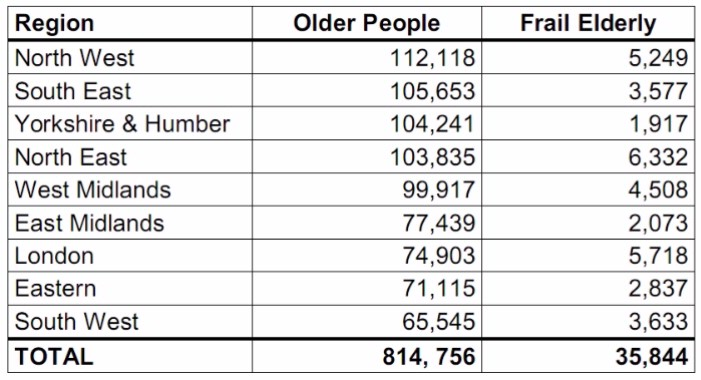
\includegraphics[width=7cm]{Images/Tables/table.jpg}\\
		
		\textbf{Result 1}\\
		Region Older People Frail Elderly

		North West 112,118 5,249\\
		South East 105,653 3,577\\
		Yorkshire \& Humber 104,241 1,917\\
		North East 103.835 6.332\\
		West Midlands 99,917 4.508\\
		East Midlands 77.439 2.073\\
		London 74,903 5.718\\
		Eastern 71.115 2.837\\
		Sou\textbf{l}h West 65,545 3,633\\
		TOTAL 814. 756 35,844\\
		
		\textbf {Table 2}\\
		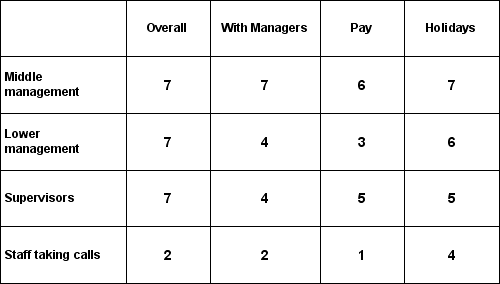
\includegraphics[width=7cm]{Images/Tables/8Table9.png}\\
		
		\textbf{Result 2}\\
		mm" with Mznzuzrs Pay Hmmzys\\
		 v 7 s 7\\
		mm 7 4 3 s
		Sllnzwlsnrs 7 4 5 5\\
		51mm...“ calls 2 2 1 4\\
		
		
		As evidenced by the sample tests above, we have not yet reached our acceptable error threshold for this system. Development will continue to improve accuracy and testing will continue concurrently.
\section{User Interface}

\section{Full System (Integration)}


\end{document}
